\documentclass[tikz, border=10pt]{standalone}
\usepackage{times}
\usepackage{pifont}
\usetikzlibrary{shapes, arrows.meta, positioning, calc, shadows, trees, backgrounds, fit, decorations.pathreplacing}

\definecolor{sedarRed}{RGB}{100, 100, 100}
\definecolor{procOrange}{RGB}{120, 120, 120}
\definecolor{ruleYellow}{RGB}{140, 140, 140}
\definecolor{noteBg}{RGB}{250, 250, 250}
\definecolor{softBlue}{RGB}{245, 245, 245}
\definecolor{borderBlue}{RGB}{70, 130, 180}
\definecolor{morphGreen}{RGB}{70, 130, 180}

\newcommand{\cmark}{\textcolor{blue}{\ding{51}}}
\newcommand{\xmark}{\textcolor{black}{\ding{55}}}

\begin{document}

\begin{tikzpicture}[
    level distance=1.0cm,
    sibling distance=2.8cm,
    font=\normalsize\ttfamily,
    edge from parent/.style={draw, -latex, gray!60, thick},
    concrete/.style={
        rectangle, draw=black!30, fill=white, rounded corners=2pt, 
        minimum height=0.7cm, align=center, drop shadow={opacity=0.05}
    },
    abstract/.style={
        rectangle, draw=blue!60, fill=blue!5, rounded corners=2pt, 
        dashed, minimum height=0.7cm, text=blue, font=\bfseries
    },
    boundary/.style={
        rectangle, draw=blue!80, fill=blue!10, rounded corners=3pt, thick, 
        minimum height=0.7cm, align=center, drop shadow={opacity=0.15, color=blue}
    },
    dialogBox/.style={
        rectangle, draw=gray!30, fill=noteBg, rounded corners=3pt, 
        font=\normalsize\sffamily, align=left, inner sep=8pt, 
        drop shadow={opacity=0.05}, text width=4.8cm, minimum height=1.6cm,
        anchor=north
    },
    pointer/.style={
        -{Circle[open, width=2.5pt, length=2.5pt]}, thick, gray!40, shorten >=3pt, dashed
    },
    cnum/.style={
        circle, draw=none, fill=gray!80, text=white, inner sep=1pt, 
        font=\bfseries\normalsize, minimum size=1.8em, yshift=-2pt
    }
]

% ============================================================
% 1. Left Tree: Source AST
% ============================================================
\begin{scope}[local bounding box=srcTree]
    \node[concrete] (root) {SELECT}
        child { node[concrete] {WHERE}
            child[sibling distance=3.0cm] { node[concrete] (op) {>}
                child { node[concrete] {u.created\_at} }
                child { 
                    node[boundary] (subRoot) {(SUBQUERY\\ROOT)} 
                    child[level distance=1.5cm] { 
                        node[concrete, font=\tiny, fill=white, opacity=0.8] (subContent) {SELECT}
                        child[level distance=0.8cm, sibling distance=1.2cm] { node[concrete, font=\tiny] {AGE(\ldots)} }
                        child[level distance=0.8cm, sibling distance=1.2cm] { node[concrete, font=\tiny] {FROM} }
                    }
                }
            }
        };
    % name=srcTitle 用于对齐右侧标题高度
    \node[above=0.2cm of root, font=\sffamily\bfseries\normalsize, color=black!70, name=srcTitle] {Source AST};
\end{scope}

% ============================================================
% 2. Engine (Center)
% ============================================================
\node[
    draw=black!60, fill=white, rounded corners=4pt, drop shadow={opacity=0.25}, 
    text width=3.8cm, inner sep=6pt, align=center
] (engine) at ($(root.east) + (5.5, -2.0)$) { 
    \textbf{\textsf{Abstraction Engine}}\\[4pt]
    \hrule height 0.5pt width 0.9\textwidth \vspace{4pt}
    \begin{tikzpicture}
        \node[
            draw=borderBlue!50, fill=softBlue, rounded corners=2pt, 
            inner sep=4pt, text width=3.2cm, align=center
        ] {
            \normalsize \textbf{Rules $\mathcal{R}$}\\[2pt]
            \renewcommand{\arraystretch}{1.2}
            \resizebox{3cm}{!}{ 
                \begin{tabular}{r c l}
                    \textcolor{black}{\texttt{AGE($\cdot$)}} & $\to$ & \textcolor{blue}{\texttt{<TimeDiff>}} \\
                    \textcolor{black}{\texttt{::INT}}        & $\to$ & \textcolor{blue}{\texttt{<TypeCast>}} \\
                    \textcolor{black}{\texttt{MIN($\cdot$)}} & $\to$ & \textcolor{blue}{\texttt{<AggMin>}} 
                \end{tabular}
            }
        };
    \end{tikzpicture}
};

% ============================================================
% 3. Right Side Content (Aligned with Engine)
% ============================================================

% 1. 确定中心序列的位置 (水平对齐 Engine)
\node[concrete, minimum width=0.9cm, anchor=west] (n1) at ($(engine.east) + (3.5, 1.0)$) {SELECT};

% 2. 序列其他部分
\node[concrete, minimum width=0.9cm, right=0.15cm of n1] (n2) {WHERE};
\node[concrete, minimum width=0.5cm, right=0.15cm of n2] (n3) {>};
\node[concrete, minimum width=1.4cm, right=0.15cm of n3] (n4) {u.created\_at};
\node[abstract, minimum width=1.3cm, below=0.3cm of n4] (n5) {<SubQuery>};
\foreach \i/\j in {1/2, 2/3, 3/4} { \draw[-latex, black!40, thick] (n\i) -- (n\j); }
\draw[-latex, black!40, thick] (n4) -- (n4 |- n5.north);
\node[left=0.1cm of n1, font=\normalsize\sffamily\bfseries, color=black!70] (snormLabel) {$S_{norm}$:};

% 3. 上方 Definition
\node[above=0.5cm of n1.west, anchor=west, font=\normalsize\sffamily, color=gray] (tupleDef) {
    Tuple $\mathcal{T} = \langle 
    \textcolor{black}{S_{norm}}, 
    \textcolor{black}{\mathcal{G}}, 
    \mathcal{D}, 
    \textcolor{black}{\mathcal{H}} 
    \rangle$
};

% 4. 下方双栏 (Graph | Segments)
\node[below=1.8cm of n1, anchor=center] (graphNode) {
    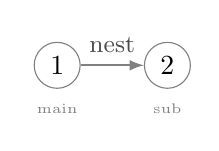
\begin{tikzpicture}[scale=0.4, baseline=0]
        \node[draw=black!50, circle, fill=white, inner sep=3pt, font=\normalsize] (g1) at (0, 0) {1};
        \node[draw=black!50, circle, fill=white, inner sep=3pt, font=\normalsize] (g2) at (3.5, 0) {2};
        \draw[-latex, thick, black!50] (g1) -- (g2) node[midway, above=1pt, font=\small, color=black!70] {nest};
        \node[below=2pt of g1, font=\tiny, color=gray] {main};
        \node[below=2pt of g2, font=\tiny, color=gray] {sub};
    \end{tikzpicture}
};
\node[left=0.1cm of graphNode, font=\normalsize\sffamily\bfseries, color=black!70] (graphLabel) {$\mathcal{G}$:};
\node[right=0.5cm of graphNode, font=\scriptsize\sffamily, color=blue] (hcLabels) {
    \textbf{$\mathcal{H}$}: \texttt{0x3f7a} \textcolor{gray}{\textit{(hash)}}
};

\node[left=0.8cm of n5, anchor=east, 
      draw=gray!30, fill=white, rounded corners=2pt, inner sep=4pt] (segBox) {
    \fontsize{9}{10}\selectfont
    \setlength{\tabcolsep}{1pt}
    \begin{tabular}{ll}
        \textcolor{black}{\textbf{ID:1}} $\to$ & [..., \textcolor{blue}{<Ptr:2>}] \\
        \textcolor{black}{\textbf{ID:2}} $\to$ & [\textcolor{blue}{<AggMin>}, ...]
    \end{tabular}
};
\node[left=0.1cm of segBox, font=\normalsize\sffamily\bfseries, color=black!70] (segLabel) {$\mathcal{D}$:};

\draw[-latex, dashed, blue, line width=0.8pt] (n5.west) to[out=-90, in=30] (segBox.east);


% 5. 绘制背景框 (Container) 
% [增加 inner ysep] 增加垂直内边距，让盒子看起来更高大
\begin{scope}[on background layer]
    \node[draw=blue, line width=1pt, dashed, rounded corners=6pt, 
          fit=(tupleDef)(snormLabel)(n5)(graphNode)(segBox)(hcLabels), 
          inner sep=22pt, inner ysep=12pt, 
          alias=aqtContainer] (aqtBox) {}; 
\end{scope}

% ============================================================
% 4. 右侧标题 (居中对齐下面的 Container)
% ============================================================
% 逻辑：取 aqtContainer.north (水平中心点)，取 srcTitle (高度)
\node[font=\bfseries\sffamily\Large, color=blue!80!black, anchor=center] 
    (aqtTitle) at (aqtContainer.north |- srcTitle) {Structure-Aware AQT};

% ============================================================
% 5. 全局连线 (Connections) 
% ============================================================

% Source -> Engine (保持水平)
\draw[-stealth, line width=1.2pt, color=black!70] (srcTree.east |- engine) -- (engine.west)
    node[midway, above=2pt, font=\normalsize\sffamily\small, text=black!80] {Input};

% Engine -> AQT (保持水平)
\draw[-stealth, line width=1.2pt, color=black!70] (engine.east) -- (aqtContainer.west |- engine.east)
    node[midway, above=2pt, font=\normalsize\sffamily\small, text=black!80] {Extract};

% ============================================================
% 6. 底部说明栏
% ============================================================
\coordinate (bottomY) at (0, -6.5);

\node[dialogBox] (step1) at (srcTree.south |- bottomY) {
    \textbf{\textcolor{blue}{Boundary Detection}}\\
    \textit{What:} Identifies query boundaries\\
    \textit{How:} Detects nested SELECT, CTE patterns
};
\node[cnum, fill=blue, left=2pt of step1.north west, anchor=north east] {1};
\draw[pointer, blue] (step1.north) to[out=90, in=-90] (subRoot.south);

\node[dialogBox] (step2) at ($(engine.south |- bottomY) + (0.6, 0)$) {
    \textbf{\textcolor{blue}{Normalizes dialect}}\\
     Applies rules $\mathcal{R}$ (e.g., AGE $\to$ \textcolor{blue}{\texttt{<TimeDiff>}})
};
\node[cnum, fill=blue, left=2pt of step2.north west, anchor=north east] {2};
\draw[pointer, blue] (step2.north) to[out=90, in=-135] (engine.south west);

\node[dialogBox] (step3) at (aqtContainer.south |- bottomY) {
    \textbf{\textcolor{blue}{Structure-Aware AQT}}\\  
    Creates matchable query representation Tuple $\mathcal{T} = \langle S_{norm}, \mathcal{G}, \mathcal{D}, \mathcal{H} \rangle$
};
\node[cnum, fill=blue, left=2pt of step3.north west, anchor=north east] {3};
\draw[pointer, blue] (step3.north) to[out=90, in=-90] (aqtContainer.south);

\node[single arrow, draw=none, fill=gray!20, % 去掉边框，用浅灰填充
      minimum height=1.0cm, minimum width=0.6cm, % 尺寸调小
      single arrow head extend=2pt] 
      at ($(step1.east)!0.5!(step2.west)$) {};

\node[single arrow, draw=none, fill=gray!20, 
      minimum height=1.0cm, minimum width=0.6cm, 
      single arrow head extend=2pt] 
      at ($(step2.east)!0.5!(step3.west)$) {};

% Discarded bits
\begin{scope}
    \tikzset{
        discarded_style/.style={
            rectangle, draw=gray!50, fill=black!10, rounded corners=2pt, 
            font=\scriptsize\ttfamily\color{black!70}, inner sep=3pt
        }
    }
    \node[discarded_style, below=0.8cm of engine.south, xshift=-0.5cm, rotate=-10] (d1) {AGE()};
    \node[discarded_style, right=0.2cm of d1, yshift=0.2cm, rotate=5] (d2) {::INT};
    
    \node[font=\normalsize\bfseries\itshape, text=gray!80, left=0.2cm of d1] {Discarded:};
    \draw[-latex, dashed, gray!60, thick] (engine.south) -- ++(0, -0.6);
\end{scope}

\end{tikzpicture}
\end{document}
